\chapter{Kiến trúc hệ thống}
\label{ch:architecture}

\section{Tổng quan kiến trúc}
Hệ thống được thiết kế và triển khai trên nền tảng AWS Singapore (\texttt{ap-southeast-1}) theo kiến trúc sẵn sàng cao đa vùng (\textit{Multi-AZ High Availability}) kết hợp nguyên tắc phòng thủ theo chiều sâu (\textit{Defense-in-Depth}) và \textit{Zero-Trust Architecture}. Điểm truy cập từ Internet được tiếp nhận tập trung qua \textbf{AWS Network Load Balancer (NLB L4)} và phân phối đều theo chế độ \textbf{Active-Active} tới cụm \textbf{Dual-Gateway} (Gateway 1 tại AZ-a và Gateway 2 tại AZ-b), trước khi lưu lượng được kiểm duyệt bởi Suricata IDS/IPS và chuyển tiếp an toàn vào cụm Kubernetes nội bộ hoặc máy chủ giám sát an ninh Wazuh SIEM chuyên biệt.

\begin{figure}[H]
    \centering
    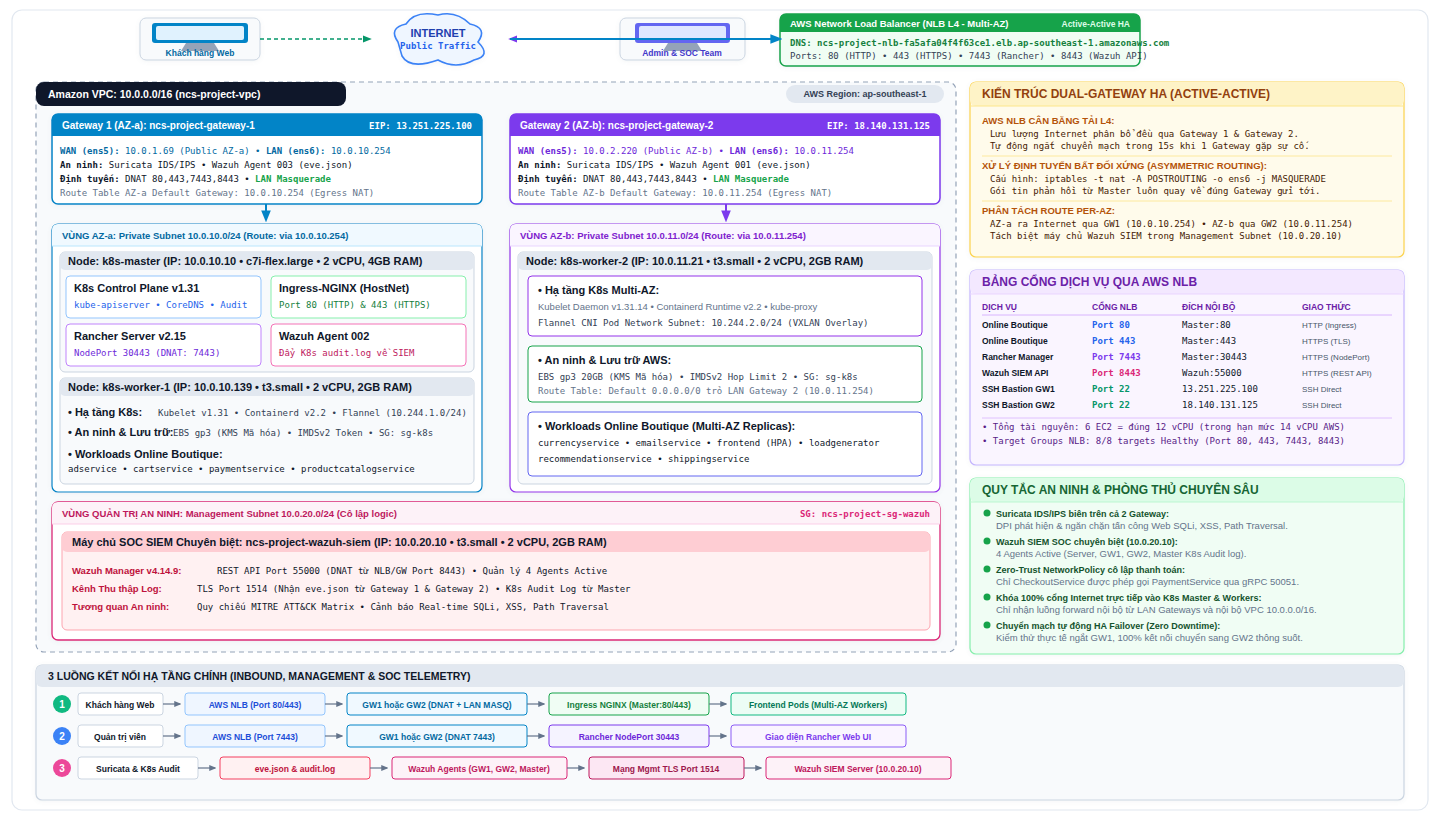
\includegraphics[width=\textwidth]{images/architecture_diagram.png}
    \caption{Sơ đồ kiến trúc tổng thể hệ thống an ninh hạ tầng Microservices trên AWS}
    \label{fig:architecture_diagram}
\end{figure}

\section{Các service ứng dụng triển khai}
Ứng dụng thương mại điện tử Google Online Boutique bao gồm 11 service độc lập kết hợp cùng 1 service sinh tải (\texttt{loadgenerator}). Các service được đóng gói dưới dạng container Docker, vận hành trên cụm Kubernetes:

\begin{table}[H]
    \centering
    \small
    \renewcommand{\arraystretch}{1.2}
    \caption{Bảng tóm tắt các service ứng dụng Online Boutique triển khai trên cụm K8s}
    \label{tab:services_summary}
    \begin{tabularx}{\textwidth}{l l c l X}
        \toprule
        \textbf{Service} & \textbf{Ngôn ngữ} & \textbf{Cổng} & \textbf{Giao thức} & \textbf{Vai trò chức năng} \\
        \midrule
        \texttt{frontend} & Go & 80, 443 & HTTP/HTTPS & Giao diện web người dùng, hiển thị trang chủ và sản phẩm \\
        \texttt{cartservice} & C\# (.NET) & 7070 & gRPC & Quản lý thông tin giỏ hàng của từng phiên người dùng \\
        \texttt{redis-cart} & Redis & 6379 & TCP & Bộ nhớ đệm in-memory lưu trữ tạm thời giỏ hàng \\
        \texttt{productcatalogservice} & Go & 3550 & gRPC & Cung cấp danh mục sản phẩm, tìm kiếm và chi tiết món đồ \\
        \texttt{checkoutservice} & Go & 5050 & gRPC & Tiếp nhận đơn hàng, điều phối thanh toán và gửi email \\
        \texttt{paymentservice} & Node.js & 50051 & gRPC & Xử lý thanh toán thẻ tín dụng (bảo vệ bởi Zero-Trust NetPol) \\
        \texttt{currencyservice} & Node.js & 7000 & gRPC & Chuyển đổi và tính toán tỷ giá ngoại tệ theo thời gian thực \\
        \texttt{emailservice} & Python & 8080 & gRPC & Soạn thảo và gửi email xác nhận đặt hàng thành công \\
        \texttt{shippingservice} & Go & 50051 & gRPC & Tính cước phí vận chuyển và xuất mã vận đơn giao hàng \\
        \texttt{recommendationservice} & Python & 8080 & gRPC & Đề xuất gợi ý các sản phẩm liên quan theo ngữ cảnh \\
        \texttt{adservice} & Java & 9555 & gRPC & Hiển thị các mẩu tin quảng cáo và khuyến mãi sản phẩm \\
        \texttt{loadgenerator} & Python & -- & HTTP & Giả lập lưu lượng truy cập liên tục để kích hoạt HPA \\
        \bottomrule
    \end{tabularx}
\end{table}

\section{Phân vùng mạng và định tuyến (VPC \& Subnets)}
Toàn bộ hạ tầng mạng được bao bọc trong một \textbf{Amazon VPC} (\texttt{ncs-project-vpc}) với dải mạng \texttt{10.0.0.0/16}. Không gian mạng được quy hoạch thành 5 Subnet độc lập trải dài trên 2 \textit{Availability Zones (AZ)}:

\begin{table}[H]
    \centering
    \small
    \renewcommand{\arraystretch}{1.25}
    \caption{Bảng phân bổ không gian địa chỉ IP và Subnet trên AWS}
    \label{tab:subnets}
    \begin{tabularx}{\textwidth}{l l l l X}
        \toprule
        \textbf{Tên Subnet} & \textbf{Vùng AZ} & \textbf{Dải CIDR} & \textbf{Loại mạng} & \textbf{Mục đích sử dụng} \\
        \midrule
        \texttt{public-wan-a} & \texttt{ap-southeast-1a} & \texttt{10.0.1.0/24} & Public & Gateway 1 (WAN \texttt{10.0.1.69} / EIP \texttt{13.251.225.100}) \\
        \texttt{public-wan-b} & \texttt{ap-southeast-1b} & \texttt{10.0.2.0/24} & Public & Gateway 2 (WAN \texttt{10.0.2.220} / EIP \texttt{18.140.131.125}) \\
        \texttt{private-subnet-a} & \texttt{ap-southeast-1a} & \texttt{10.0.10.0/24} & Private & K8s Master (\texttt{10.0.10.10}) và Worker 1 (\texttt{10.0.10.139}) \\
        \texttt{private-subnet-b} & \texttt{ap-southeast-1b} & \texttt{10.0.11.0/24} & Private & K8s Worker 2 (\texttt{10.0.11.21}) \\
        \texttt{mgmt-subnet} & \texttt{ap-southeast-1a} & \texttt{10.0.20.0/24} & Private & Máy chủ SOC Wazuh SIEM chuyên biệt (\texttt{10.0.20.10}) \\
        \bottomrule
    \end{tabularx}
\end{table}

\subsection{Bảng định tuyến per-AZ và Cơ chế phân giải định tuyến bất đối xứng}
\begin{enumerate}
    \item \textbf{Public Route Table}: Liên kết với \texttt{public-wan-a} và \texttt{public-wan-b}, định tuyến \texttt{0.0.0.0/0} hướng trực tiếp ra \textit{Internet Gateway} (\texttt{igw}).
    \item \textbf{Private Route Table AZ-a}: Liên kết với \texttt{private-subnet-a} và \texttt{mgmt-subnet}. Quy tắc \texttt{0.0.0.0/0} trỏ đích đến Network Interface LAN của Gateway 1 (\texttt{10.0.10.254}), phục vụ egress internet cho Master, Worker 1 và Wazuh SIEM.
    \item \textbf{Private Route Table AZ-b}: Liên kết với \texttt{private-subnet-b}. Quy tắc \texttt{0.0.0.0/0} trỏ đích đến Network Interface LAN của Gateway 2 (\texttt{10.0.11.254}), phục vụ egress internet độc lập cho Worker 2.
    \item \textbf{Giải quyết Asymmetric Routing (LAN Masquerade)}: Nhằm đảm bảo các gói tin DNAT từ Gateway 2 tới Master không bị Master phản hồi lệch qua Gateway 1, cả hai Gateway đều kích hoạt luật:
    \begin{lstlisting}[language=bash]
    iptables -t nat -A POSTROUTING -o ens6 -j MASQUERADE
    \end{lstlisting}
    Luật này tự động chuyển đổi địa chỉ IP nguồn thành IP LAN của chính Gateway đó, bảo đảm gói tin trả về đi đúng tuyến đối xứng.
\end{enumerate}

\section{Security Groups và Kiểm soát truy cập}
Hạ tầng áp dụng 3 Security Group độc lập theo nguyên tắc đặc quyền tối thiểu (\textit{Least Privilege}):
\begin{itemize}
    \item \textbf{\texttt{ncs-project-sg-pfsense}}: Áp dụng cho 2 Edge Gateway. Mở các cổng công khai từ Internet: cổng 80 (HTTP), cổng 443 (HTTPS), cổng 7443 (Rancher), cổng 8443 (Wazuh SIEM API) và cổng 22 (SSH).
    \item \textbf{\texttt{ncs-project-sg-k8s}}: Áp dụng cho Master node và Worker nodes. \textbf{Khóa 100\% truy cập trực tiếp từ Internet}. Chỉ chấp nhận lưu lượng chuyển tiếp nội bộ đến từ card mạng LAN của các Gateway (\texttt{10.0.10.254}, \texttt{10.0.11.254}) qua các cổng dịch vụ 80, 443, 6443, 9443, 30000--32767 và thông suốt nội bộ dải \texttt{10.0.0.0/16}.
    \item \textbf{\texttt{ncs-project-sg-wazuh}}: Áp dụng cho máy chủ chuyên biệt Wazuh SIEM. Cho phép nhận traffic thu thập log Agent (1514, 1515 TCP/UDP) và REST API (55000) từ dải mạng nội bộ VPC.
\end{itemize}

\section{Bảng ánh xạ cổng service và cơ chế NAT (Port Mapping Table)}
Toàn bộ lưu lượng công khai từ Internet đi qua \textbf{AWS Network Load Balancer (NLB L4)} cân bằng tải đều tới Gateway 1 và Gateway 2. Tại mỗi Gateway, IPTables DNAT và LAN Masquerade chuyển tiếp vào mạng nội bộ:

\begin{table}[H]
    \centering
    \small
    \renewcommand{\arraystretch}{1.25}
    \caption{Bảng phân bổ cổng service và quy tắc chuyển tiếp NAT}
    \label{tab:port_mapping}
    \begin{tabularx}{\textwidth}{l c c l X}
        \toprule
        \textbf{Tên service} & \textbf{Cổng NLB} & \textbf{Giao thức} & \textbf{Đích Internal (DNAT)} & \textbf{Mô Tả} \\
        \midrule
        \textbf{Online Boutique (HTTP)} & \textbf{80} & HTTP & \texttt{10.0.10.10:80} & Ứng dụng web thương mại điện tử \\
        \textbf{Online Boutique (HTTPS)} & \textbf{443} & HTTPS & \texttt{10.0.10.10:443} & Giao diện web mã hóa bảo mật TLS \\
        \textbf{Rancher Server} & \textbf{7443} & HTTPS & \texttt{10.0.10.10:30443} & Giao diện quản trị tập trung cụm K8s \\
        \textbf{Wazuh SIEM API} & \textbf{8443} & HTTPS & \texttt{10.0.20.10:55000} & Giao tiếp REST API \& Giám sát an ninh \\
        \textbf{SSH Bastion GW1} & \textbf{22} & SSH & Trực tiếp Gateway 1 & Quản trị dòng lệnh qua IP \texttt{13.251.225.100} \\
        \textbf{SSH Bastion GW2} & \textbf{22} & SSH & Trực tiếp Gateway 2 & Quản trị dòng lệnh qua IP \texttt{18.140.131.125} \\
        \bottomrule
    \end{tabularx}
\end{table}

\section{Mạng Pod Overlay (Flannel VXLAN)}
Cụm Kubernetes sử dụng CNI \textbf{Flannel}:
\begin{itemize}
    \item Mỗi node trong cụm được phân bổ một không gian con \texttt{/24} (Master \texttt{10.244.0.0/24}, Worker 1 \texttt{10.244.1.0/24}, Worker 2 \texttt{10.244.2.0/24}).
    \item Gói tin trao đổi giữa các Pod được đóng gói trong giao thức UDP port 8472 trên card mạng nội bộ, cho phép các Pod thuộc 12 service giao tiếp với nhau giữa 2 vùng (\texttt{ap-southeast-1a} và \texttt{ap-southeast-1b}).
\end{itemize}

\section{Máy chủ EC2}
Hạ tầng tính toán sử dụng 6 máy chủ EC2 với tổng lượng CPU là 12 vCPU, hoàn toàn nằm trong hạn mức 14 vCPU của tài khoản AWS Singapore:

\begin{table}[H]
    \centering
    \small
    \renewcommand{\arraystretch}{1.25}
    \caption{Bảng phân bổ máy chủ EC2 trong hệ thống}
    \label{tab:ec2_resources}
    \begin{tabularx}{\textwidth}{l l c c c X}
        \toprule
        \textbf{Máy chủ (Host)} & \textbf{Loại Instance} & \textbf{vCPU} & \textbf{RAM} & \textbf{EBS Disk} & \textbf{Nhiệm vụ chính} \\
        \midrule
        \texttt{pfsense-gateway-1} & \texttt{t3.small} & 2 & 2 GB & 20 GB (gp3) & Gateway AZ-a, Suricata IDS/IPS, NAT, Bastion \\
        \texttt{pfsense-gateway-2} & \texttt{t3.small} & 2 & 2 GB & 20 GB (gp3) & Gateway AZ-b, Suricata IDS/IPS, NAT, Bastion \\
        \texttt{k8s-master} & \texttt{c7i-flex.large} & 2 & 4 GB & 20 GB (gp3) & K8s Control Plane, Ingress-NGINX, Rancher \\
        \texttt{k8s-worker-1} & \texttt{t3.small} & 2 & 2 GB & 20 GB (gp3) & K8s Worker node AZ-a \\
        \texttt{k8s-worker-2} & \texttt{t3.small} & 2 & 2 GB & 20 GB (gp3) & K8s Worker node AZ-b \\
        \texttt{wazuh-siem} & \texttt{t3.small} & 2 & 2 GB & 20 GB (gp3) & Máy chủ chuyên biệt Wazuh SIEM Manager (SOC) \\
        \midrule
        \textbf{Tổng cộng} & \textbf{6 EC2} & \textbf{12} & \textbf{14 GB} & \textbf{120 GB} & \textbf{Hạn mức: 12/14 vCPU (Singapore)} \\
        \bottomrule
    \end{tabularx}
\end{table}
